\newcommand{\psd}[1]{{\small\sffamily{\color{blue!60}#1}}}



The problem of interest is a single Dirichlet condition (clamped end
bar) and traction loading. For this example we use Newmark-\(\beta\)
time discretization. Additionally postrocessing is demanded for
displacement, acceleration, and velocity (\(u,a,v\)).

\begin{lstlisting}[style=BashInputStyle]
PSD_PreProcess -dimension 2 -problem elastodynamics -dirichletconditions 1 -tractionconditions 1 \
-timediscretization newmark_beta -postprocess uav
\end{lstlisting}

Once the step above has been performed, we solve the problem using two
MPI processes, with the given mesh file \psd{bar-dynamic.msh}.

\begin{lstlisting}[style=BashInputStyle]
PSD_Solve -np 2 Main.edp -mesh ./../Meshes/2D/bar-dynamic.msh -v 0
\end{lstlisting}

\begin{figure}[h!]
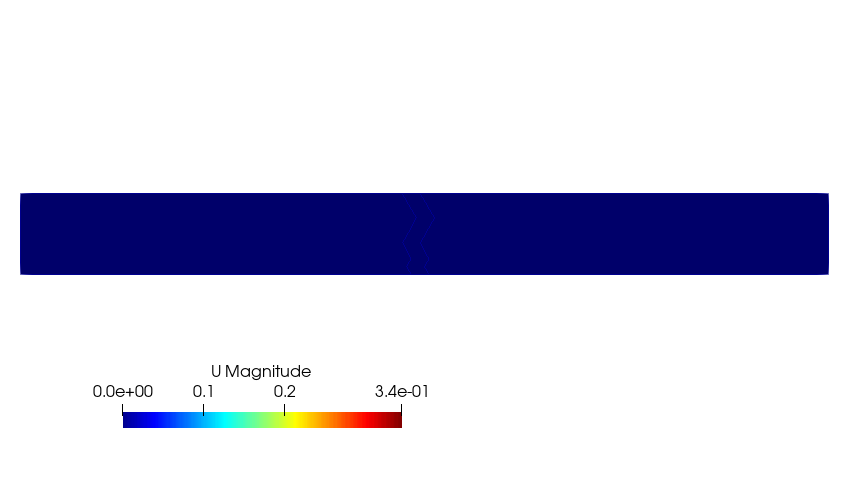
\includegraphics[width=0.19\textwidth]{./Images/ed-u0.png}
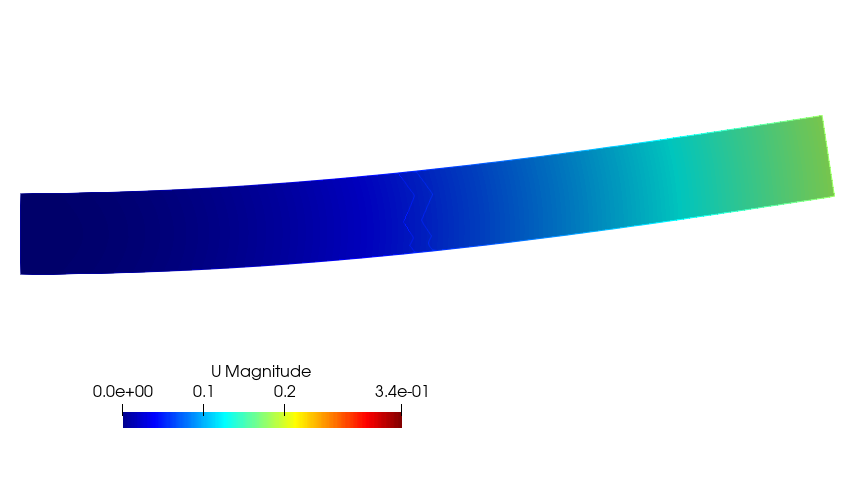
\includegraphics[width=0.19\textwidth]{./Images/ed-u2.png}
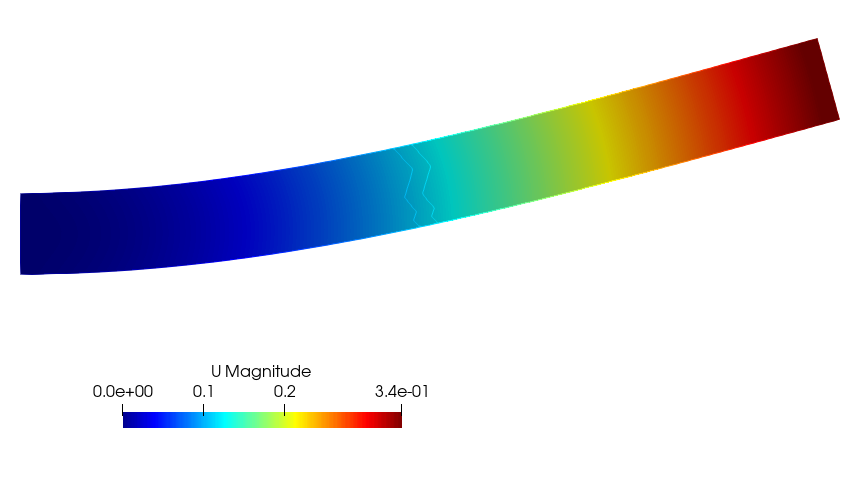
\includegraphics[width=0.19\textwidth]{./Images/ed-u3.png}
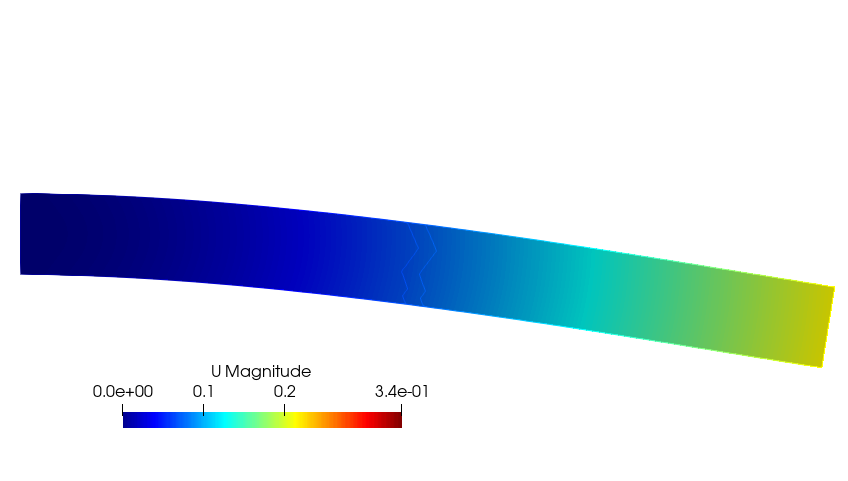
\includegraphics[width=0.19\textwidth]{./Images/ed-u4.png}
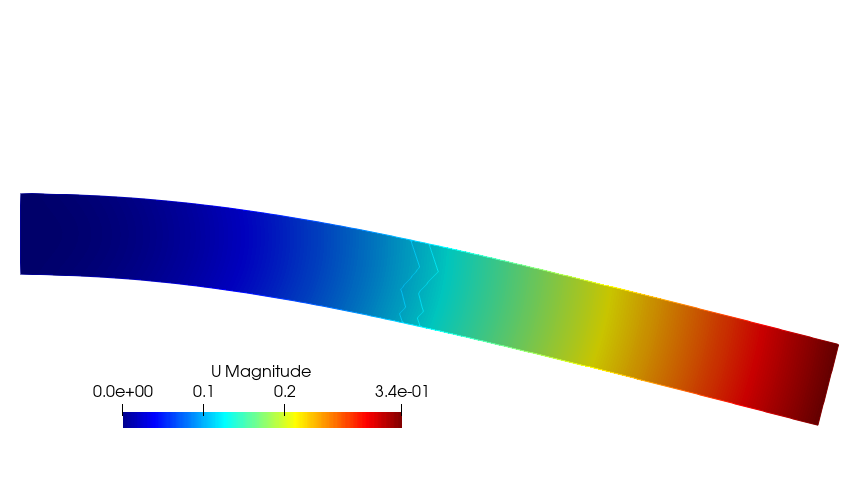
\includegraphics[width=0.19\textwidth]{./Images/ed-u5.png}
\caption{Finite element displacement field on warped mesh shown at different time steps. \label{bar-ed}}
\end{figure}

Using ParaView for postprocessing the results that are provided in the
\psd{VTUs...} folder, results such as those shown in
figure\textasciitilde{}\ref{bar-ed} can be extracted.
